\documentclass[11pt,a4paper]{article}
\usepackage[margin=2.4cm]{geometry}
\usepackage{amsmath,amssymb,amsthm,bm}
\usepackage{graphicx}
\usepackage{booktabs}
\usepackage{xcolor}
\usepackage[colorlinks=true,linkcolor=blue!60!black,citecolor=blue!60!black]{hyperref}
\usepackage{caption}
\captionsetup{font=small,labelfont=bf}

\newtheorem{proposition}{Proposition}
\newtheorem{definition}{Definition}
\theoremstyle{remark}
\newtheorem{remark}{Remark}

\newcommand{\uu}{\bm{u}}
\newcommand{\nn}{\bm{n}}
\newcommand{\ttt}{\bm{t}}
\newcommand{\Sf}{\bm{S}}
\newcommand{\rAU}{r_{A_U}}
\newcommand{\rAtU}{r_{A_tU}}
\newcommand{\dd}{\,\mathrm{d}}

\title{\bf A cut-cell immersed-boundary method for free-slip and no-slip walls\\
\large Formulation, properties and verification}
\author{}
\date{\today}

\begin{document}
\maketitle

\begin{abstract}
We describe an immersed-boundary method for free-slip (perfect-slip) walls in a
collocated finite-volume solver for the incompressible Navier--Stokes equations. The
boundary is represented by a level set; each face of the Cartesian mesh carries the
fraction of its area that lies in the fluid, and each cell the fraction of its volume. The
free-slip condition is not imposed at any point of the discretisation: it is carried
entirely by a geometric closure identity relating the partially open faces of a cut cell to
its wall segment. As a consequence the method requires no ghost values, no extrapolation
into the solid, and no coupling between the velocity components. We prove that the
discretisation is exact for uniform flow parallel to a plane wall of arbitrary orientation,
that it generates no spurious force from a uniform pressure field, and that no-penetration
follows from discrete continuity rather than being imposed. The same construction serves a
no-slip wall by restoring a single term, the viscous traction of the wall segment, which is
the only quantity the free-slip condition sets to zero. Measured against exact solutions on a
curved boundary, the method is \emph{second order} for free slip and \emph{first order} for
no slip; we identify the wall-normal distance estimate required by no slip, and not by free
slip, as the cause of the difference.
\end{abstract}

\tableofcontents

\section{Scope and notation}

We consider the incompressible Navier--Stokes equations
\begin{equation}
\frac{\partial \uu}{\partial t}+\nabla\!\cdot\!(\uu\uu)-\nabla\!\cdot\!(\nu\nabla\uu)
=-\nabla p+\bm{g},
\qquad \nabla\!\cdot\!\uu=0,
\label{eq:ns}
\end{equation}
with $p$ the reduced (kinematic) pressure and $\bm{g}$ a body force, in a two-dimensional
domain $\Omega$ containing a stationary rigid body $B$. On $\partial B$ we impose the
\emph{free-slip} conditions
\begin{equation}
\uu\cdot\nn = 0,
\qquad
\big(\bm{\tau}\cdot\nn\big)\cdot\ttt = 0,
\label{eq:bc}
\end{equation}
that is, no penetration together with vanishing tangential traction; $\nn$ and $\ttt$ are the
unit normal and tangent of $\partial B$ and $\bm{\tau}$ the viscous stress. For a Newtonian
fluid the second condition is $\partial u_t/\partial n = O(\kappa u_t)$, and to the order
retained here it is $\partial u_t/\partial n = 0$.

The mesh is uniform and Cartesian with spacings $\Delta x,\Delta y$ and cell volume
$V=\Delta x\Delta y$; all variables are stored at cell centres. For a cell $P$ we write
$\mathcal F(P)=\{E,W,N,S\}$ for its four faces, $A_f$ for the face area
($A_f=\Delta y$ on $x$-faces, $\Delta x$ on $y$-faces), $\nn_f$ for the outward unit normal
and $h_f$ for the centre-to-centre distance across $f$.

\section{Geometric description of the boundary}

\begin{definition}[Level set]
The body is given by a function $\varphi:\Omega\to\mathbb R$ with
$\varphi<0$ inside $B$, $\varphi>0$ in the fluid and $\varphi=0$ on $\partial B$. Only the
sign of $\varphi$ and the location of its zero level are used; $\varphi$ need not be a signed
distance.
\end{definition}

\begin{definition}[Fluid fractions]
For each face $f$ let
\begin{equation}
\theta_f=\frac{1}{A_f}\big|\{\bm{x}\in f:\varphi(\bm{x})>0\}\big| \in[0,1],
\end{equation}
the fraction of the face lying in the fluid, and for each cell $P$
\begin{equation}
\alpha_P=\frac{1}{V}\big|\{\bm{x}\in P:\varphi(\bm{x})>0\}\big| \in[0,1].
\end{equation}
A cell is \emph{fluid} if $\alpha_P=1$, \emph{solid} if $\alpha_P=0$ and \emph{cut} otherwise.
\end{definition}

The fluid part of a cut cell is a polygon $P^{\rm f}$ whose boundary consists of the
partially open axis faces, of area $\theta_fA_f$, together with the wall segment
$\partial B\cap P$, of area $A_{\rm wall}$ and outward unit normal $\nn_{\rm wall}$
(Fig.~\ref{fig:cutcell}).

\begin{figure}[t]\centering
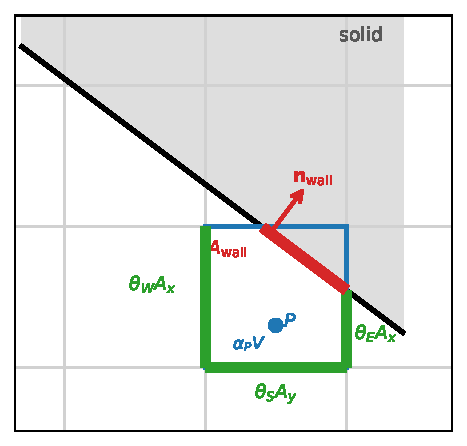
\includegraphics[width=0.60\textwidth]{figs2/f1_cutcell.pdf}
\caption{A cut cell. Its fluid boundary consists of the partially open axis faces (green,
areas $\theta_fA_f$) and the wall segment (red, area $A_{\rm wall}$, outward normal
$\nn_{\rm wall}$). The cell carries fluid volume $\alpha_PV$.}
\label{fig:cutcell}
\end{figure}

\begin{figure}[t]\centering
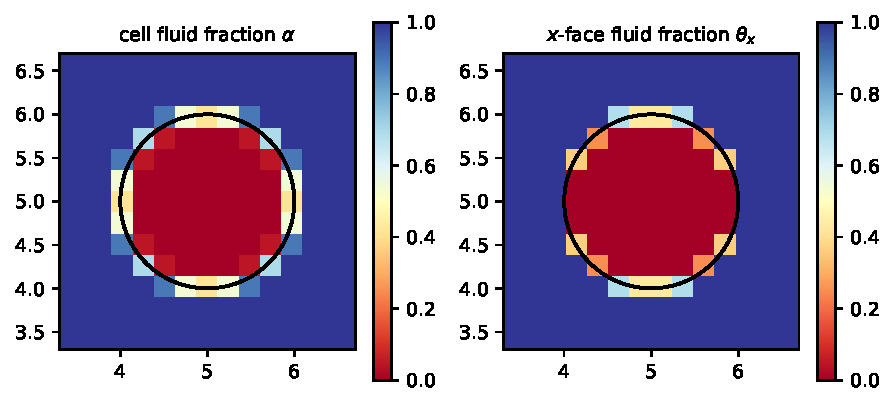
\includegraphics[width=0.94\textwidth]{figs2/f2_fractions.pdf}
\caption{Fluid fractions for a circular cylinder on a $41\times41$ mesh: cell fractions
$\alpha$ (left) and $x$-face fractions $\theta_x$ (right). The boundary is resolved by the
fractions alone; no marker points or surface triangulation are used.}
\label{fig:fractions}
\end{figure}

\subsection{The closure identity}

\begin{proposition}[Geometric closure]
\label{prop:closure}
For every cut cell,
\begin{equation}
\sum_{f\in\mathcal F(P)}\theta_f\,\nn_f A_f \;+\; \nn_{\rm wall}A_{\rm wall}\;=\;\bm 0 .
\label{eq:closure}
\end{equation}
\end{proposition}

\begin{proof}
Apply the divergence theorem to the constant vector field $\bm{e}_i$ over the closed region
$P^{\rm f}$: $\int_{P^{\rm f}}\nabla\!\cdot\!\bm{e}_i\dd V=0=\oint_{\partial P^{\rm f}}
\bm{e}_i\cdot\nn\dd S$. Since $\partial P^{\rm f}$ consists exactly of the wet portions of
the axis faces and the wall segment, and the wet portion of face $f$ has area $\theta_fA_f$
and constant normal $\nn_f$, the surface integral is
$\bm{e}_i\cdot\big(\sum_f\theta_f\nn_fA_f+\nn_{\rm wall}A_{\rm wall}\big)$. As this vanishes
for $i=1,2$, \eqref{eq:closure} follows.
\end{proof}

\begin{remark}
In the implementation $\nn_{\rm wall}A_{\rm wall}$ is never computed independently: it is
\emph{defined} by \eqref{eq:closure}. The identity therefore holds to machine precision by
construction, and the wall orientation is inherited from the same fractions that weight the
faces. Evaluated on a plane wall inclined at $45^\circ$ to the mesh, the normal recovered
from \eqref{eq:closure} agrees with the analytic normal to $2.2\times10^{-16}$.
\end{remark}

\section{Discretisation}

\subsection{Face fluxes}
The volume flux through the wet part of a face is
\begin{equation}
\phi_f=\theta_f\,A_f\,\big(\bar\uu_f\cdot\nn_f\big),
\qquad \bar\uu_f=\tfrac12\big(\uu_P+\uu_{nb}\big).
\label{eq:flux}
\end{equation}

\subsection{The four terms}
Each term of \eqref{eq:ns} is integrated over $P^{\rm f}$. The wall segment contributes to
each according to \eqref{eq:bc}, and this is where the boundary condition enters --- nowhere
else. Table~\ref{tab:terms} collects the result.

\begin{table}[h]\centering
\caption{Contribution of the wall segment to each term, and the resulting discrete operator.
$\Gamma$ denotes the diffusivity, $p_f=\frac12(p_P+p_{nb})$.}
\label{tab:terms}
\small
\begin{tabular}{@{}p{2.3cm}p{5.4cm}p{6.6cm}@{}}
\toprule
term & wall contribution & discrete operator\\
\midrule
unsteady & --- &
$\dfrac{\alpha_PV}{\Delta t}\big(\uu_P^{n+1}-\uu_P^{n}\big)$\\[6pt]
viscous &
zero: free slip gives no tangential traction, and the normal viscous traction is
$O(\Delta)$ &
$\displaystyle\sum_f \theta_f\,\Gamma_f\,\frac{\uu_{nb}-\uu_P}{h_f}A_f$\\[10pt]
convective &
zero: $\uu\cdot\nn_{\rm wall}=0$ carries no flux &
$\displaystyle\sum_f \phi_f\,\bar\uu_f$\\[10pt]
pressure &
$p_{\rm wall}\,\nn_{\rm wall}A_{\rm wall}$ --- the form drag; $p_{\rm wall}=p_P+O(\Delta)$ &
$\displaystyle\sum_f \theta_f\,(p_f-p_P)\,\nn_f A_f$\\[10pt]
continuity & zero &
$\displaystyle\sum_f \phi_f = 0$\\
\bottomrule
\end{tabular}
\end{table}

The pressure entry deserves a derivation. The volume-integrated pressure gradient is
$\oint_{\partial P^{\rm f}}p\,\nn\dd S$. Splitting the boundary and using
$p_{\rm wall}=p_P$,
\begin{equation}
\oint p\,\nn\dd S=\sum_f\theta_f p_f\nn_fA_f+p_P\,\nn_{\rm wall}A_{\rm wall}
\overset{\eqref{eq:closure}}{=}\sum_f\theta_f p_f\nn_fA_f-p_P\sum_f\theta_f\nn_fA_f
=\sum_f\theta_f\,(p_f-p_P)\,\nn_fA_f .
\label{eq:grad}
\end{equation}
The wall force is thus absorbed exactly into the face sum; it is not dropped.

\section{Properties}

\begin{proposition}[Exactness for uniform tangential flow]
\label{prop:exact}
Let the wall be plane with normal $\nn_{\rm wall}$, and let the discrete velocity be uniform,
$\uu_P=\uu_{nb}=\uu$ with $\uu\cdot\nn_{\rm wall}=0$. Then the discrete divergence vanishes
identically in every cut cell.
\end{proposition}
\begin{proof}
From \eqref{eq:flux}, $\bar\uu_f=\uu$ and
$\sum_f\phi_f=\uu\cdot\sum_f\theta_f\nn_fA_f
\overset{\eqref{eq:closure}}{=}-\uu\cdot\nn_{\rm wall}A_{\rm wall}=0$.
\end{proof}

\begin{proposition}[No spurious force from a uniform pressure]
If $p$ is constant then the discrete pressure gradient \eqref{eq:grad} is exactly zero in
every cell, cut or not.
\end{proposition}
\begin{proof}
$p_f-p_P=0$ for every face.
\end{proof}

\begin{proposition}[No-penetration is implied, not imposed]
\label{prop:nopen}
Let $\uu$ be locally uniform in a cut cell with $A_{\rm wall}\neq0$. Then discrete continuity
$\sum_f\phi_f=0$ holds if and only if $\uu\cdot\nn_{\rm wall}=0$.
\end{proposition}
\begin{proof}
As in Proposition~\ref{prop:exact}, $\sum_f\phi_f=-\uu\cdot\nn_{\rm wall}A_{\rm wall}$.
\end{proof}

Proposition~\ref{prop:nopen} is the structural point of the method. The first of the two
boundary conditions \eqref{eq:bc} is never written down; it is a consequence of enforcing
mass conservation on the cut cell. The second appears only as the \emph{absence} of a wall
term in the viscous operator. Consequently the discretisation contains
\begin{itemize}\itemsep2pt
\item no ghost value and no extrapolation into the solid,
\item no blanking of cut cells: every cell with $\alpha_P>0$ carries its equations,
\item no coupling between the velocity components introduced by the boundary, so the
      momentum equations remain two independent scalar problems,
\item no free parameter of any kind in the boundary treatment.
\end{itemize}

\section{Pressure--velocity coupling and the algorithm}

Time advance is implicit Euler used as pseudo-transient continuation; the coupling is SIMPLEC
in the form used by OpenFOAM's \texttt{simpleFoam}. Writing the assembled momentum equation
as $a_P\uu_P=H(\uu)-V\nabla p$ with $H(\uu)=b-\sum_{nb}a_{nb}\uu_{nb}$,
\begin{equation}
\rAU=\frac{1}{a_P},\qquad
\rAtU=\frac{1}{a_P+\sum_{nb}a_{nb}},\qquad
\nabla\!\cdot\!\big(\rAtU V\nabla p\big)=\nabla\!\cdot\!\phi_{H/a_P},
\end{equation}
with the Laplacian and its flux both weighted by $\theta$, consistently. Solid cells
($\alpha_P=0$) carry no equation and are given an identity row.

\paragraph{Constant flow rate.}
A free-slip body exerts no friction, so a prescribed body force admits no steady state: the
flow accelerates without bound. The bulk velocity is therefore prescribed and the force
follows. Since only the source depends on $g_x$ and one predictor--projection pass is affine
in it, two passes give the exact value
\begin{equation}
g_x=\frac{U_b^{\rm target}-U_b^{(0)}}{U_b^{(1)}-U_b^{(0)}},
\end{equation}
where $U_b^{(0)}$, $U_b^{(1)}$ are the bulk velocities obtained with $g_x=0$ and $g_x=1$.
No relaxation parameter is involved and both passes share the matrix factorisations.

\begin{figure}[t]\centering
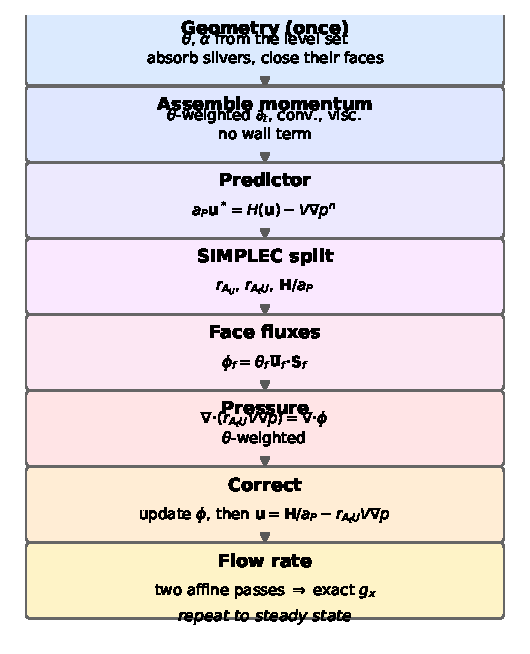
\includegraphics[width=0.44\textwidth]{figs2/f3_algorithm.pdf}
\caption{One outer iteration. The geometry is computed once; everything below it is repeated
until the residual stalls at the solver tolerance.}
\label{fig:algo}
\end{figure}

\section{Implementation}

\paragraph{Fluid fractions.}
$\theta_f$ is obtained by bisection along the face: the level set is evaluated at the two
endpoints and, when they differ in sign, the crossing is located to machine precision.
$\alpha_P$ is obtained by sub-sampling the level set on an $n_{\rm sub}\times n_{\rm sub}$
lattice within the cell ($n_{\rm sub}=32$ here). Both are computed once, before the time loop.

\paragraph{Small cells.} Cut cells with $\alpha_P\to0$ carry vanishing volume against faces of
size $O(\Delta)$, the classic small-cell problem of cut-cell methods. Cells with
$\alpha_P<\alpha_{\min}$ are absorbed into the body. This displaces the boundary by
$O(\alpha_{\min}\Delta)$, within the first-order error of the scheme. Cell merging would
remove even this perturbation.

Two conditions must be respected for Proposition~\ref{prop:closure} to survive
implementation, and both are silent failures if violated.

\begin{description}
\item[C1.] \emph{An absorbed cell must have its faces closed as well as its volume zeroed.}
Setting $\alpha_P=0$ while leaving $\theta_f>0$ on its faces breaks \eqref{eq:closure} for the
\emph{neighbouring} cells; the divergence of the exact uniform field then degrades from $0$ to
$O(\Delta)$.
\item[C2.] \emph{On a periodic mesh the faces at $x=0$ and $x=L_x$ are the same face} (and
likewise in $y$). Evaluating $\theta$ independently at both leaves an inconsistent seam and
destroys global conservation. The fraction is computed once and copied. The same requirement
applies to the level set of a test geometry: a plane oblique wall must be defined through the
periodic difference $d=\mathrm{mod}(y-x+L_y/2,\,L_y)-L_y/2$, or it does not close on the
torus.
\end{description}

\section{Verification}

\subsection{Operator level}
The exact solution of a plane free-slip channel inclined at $45^\circ$ to the mesh is uniform
flow parallel to the walls at zero driving force. Substituting it into each discrete operator
gives, on an $81\times81$ mesh,

\begin{table}[h]\centering
\caption{Residual of each operator applied to the exact solution. Values are the maxima over
all fluid cells.}
\label{tab:oplevel}
\begin{tabular}{lc}
\toprule
operator & residual\\
\midrule
discrete divergence $\sum_f\phi_f$      & $0.000\times10^{0}$\\
viscous operator                        & $0.000\times10^{0}$\\
convective operator                     & $0.000\times10^{0}$\\
pressure gradient of a uniform field    & $0.000\times10^{0}$\\
\bottomrule
\end{tabular}
\end{table}

\subsection{Solver level: the oblique channel}
Solving the full system on the same geometry, the computed driving force and velocity spread
are at the level of the linear-solver tolerance:

\begin{table}[h]\centering
\caption{Oblique free-slip channel, $\nu=1$. Exact answer: uniform flow, $g_x=0$. All cases
converged to a residual of $10^{-9}$.}
\label{tab:ch45}
\begin{tabular}{lccc}
\toprule
$n_x$ & drag $g_xA_{\rm fluid}$ & mean $|\nabla\!\cdot\!\phi|$, fluid & mean $|\nabla\!\cdot\!\phi|$, solid\\
\midrule
41 & $0.000000$ & $4.7\times10^{-18}$ & $0$\\
81 & $0.000000$ & $2.2\times10^{-18}$ & $0$\\
\bottomrule
\end{tabular}
\end{table}

\subsection{Solver level: circular cylinder}
A free-slip circular cylinder of radius $R=1$ sits at the centre of a $10\times10$ doubly
periodic box; the flow is driven at fixed bulk velocity $U_b=0.5$. The drag equals
$g_xA_{\rm fluid}$ at steady state.

\begin{table}[h]\centering
\caption{Free-slip cylinder. All cases converged to a residual of $10^{-9}$; the discrete
continuity error is at round-off and the up--down symmetry of the solution is preserved to
$10^{-14}$.}
\label{tab:cyl}
\begin{tabular}{lccccc}
\toprule
$n_x$ & 41 & 61 & 81 & 121 & fitted $\Delta\to0$\\
$\Delta$ & 0.2439 & 0.1639 & 0.1235 & 0.0826 & \\
\midrule
$\nu=1.0$\ \ ($Re_R=0.5$) & 2.829667 & 2.907463 & 2.938772 & 2.977790 & 3.038685\\
$\nu=0.5$\ \ ($Re_R=1.0$) & 1.449213 & 1.487457 & 1.503127 & 1.523026 & 1.556346\\
\bottomrule
\end{tabular}
\end{table}

Fitting $f(\Delta)=f_0-C\Delta^{p}$ by least squares over the four meshes gives
\begin{equation}
p=1.12\ \ (\nu=1),\qquad p=1.06\ \ (\nu=0.5),
\end{equation}
with r.m.s.\ residuals of $1.9\times10^{-3}$ and $9.5\times10^{-4}$ respectively
(Fig.~\ref{fig:conv}). The scheme is thus first-order accurate in the drag, consistently at
both Reynolds numbers, as expected from the $O(\Delta)$ placement of the boundary in the
pressure and viscous wall terms.

\begin{figure}[t]\centering
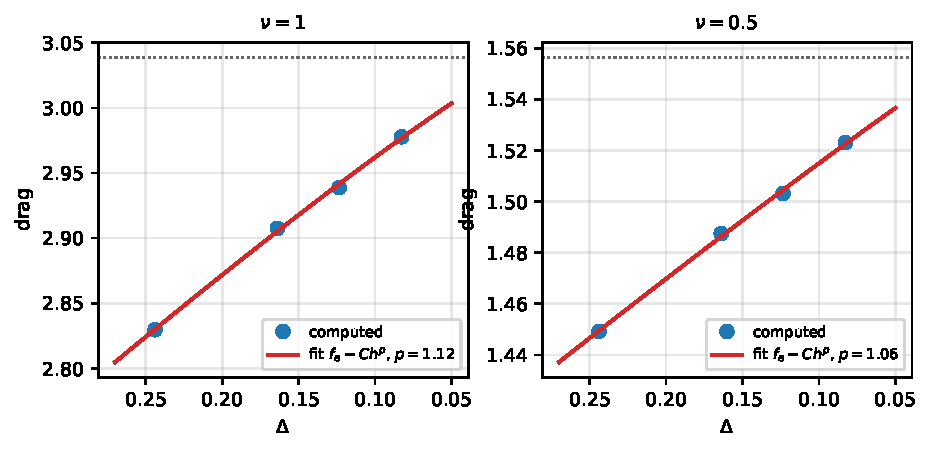
\includegraphics[width=0.94\textwidth]{figs2/f4_convergence.pdf}
\caption{Cylinder drag against mesh spacing with the least-squares fit $f_0-C\Delta^p$. The
dotted line marks the extrapolated $\Delta\to0$ value.}
\label{fig:conv}
\end{figure}

\begin{figure}[t]\centering
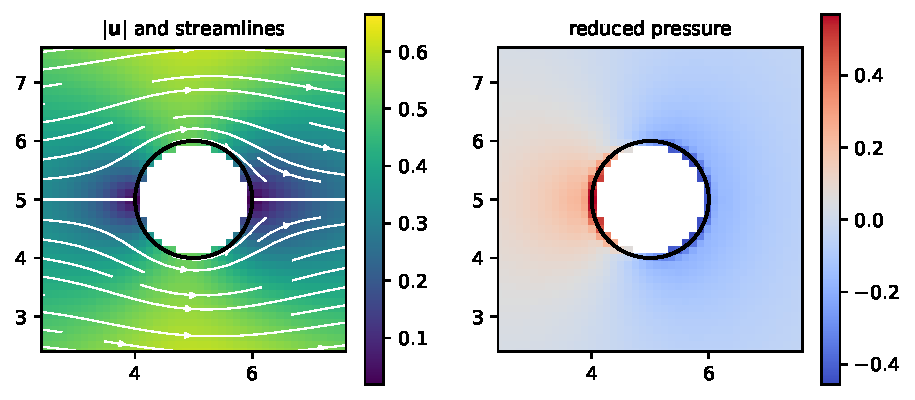
\includegraphics[width=0.96\textwidth]{figs2/f5_field.pdf}
\caption{Converged solution at $n_x=81$, $\nu=0.5$: velocity magnitude with streamlines
(left) and reduced pressure (right). The flow slides along the surface and remains attached.}
\label{fig:field}
\end{figure}

\begin{figure}[t]\centering
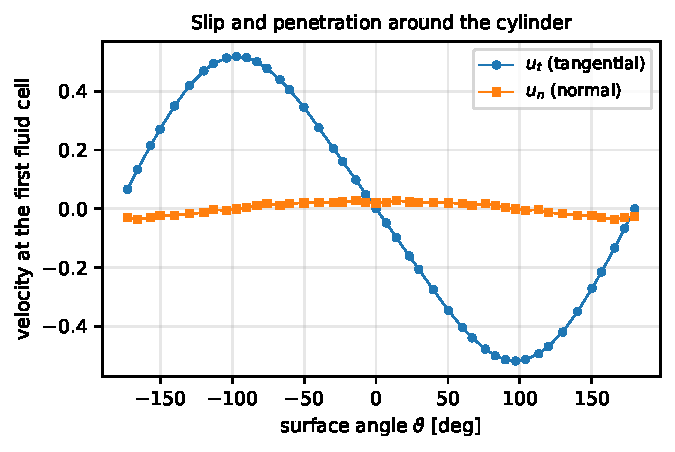
\includegraphics[width=0.56\textwidth]{figs2/f6_slip.pdf}
\caption{Tangential and normal velocity at the first fluid cell around the cylinder. The
tangential component is $O(U)$, as free slip requires; the cell-centred normal component is
not identically zero (see Sec.~\ref{sec:limits}), though the face fluxes through the boundary
are.}
\label{fig:slip}
\end{figure}


\section{No-slip walls}\label{sec:noslip}

Of the four terms in Table~\ref{tab:terms}, exactly one is set to zero by the free-slip
condition rather than by geometry: the viscous traction of the wall segment. Restoring it
gives a no-slip wall and changes nothing else.

With $\uu_{\rm wall}=\bm 0$ and a profile linear in the wall-normal direction,
\begin{equation}
\int_{\rm wall}\nu\,\frac{\partial \uu}{\partial n}\dd S \;\simeq\;
\nu\,\frac{\bm 0-\uu_P}{d}\,A_{\rm wall},
\qquad
d=\frac{\alpha_PV}{2A_{\rm wall}} .
\label{eq:noslip}
\end{equation}
The distance $d$ requires no new geometry: a wall-adjacent cell holds fluid of volume
$\alpha_PV$ behind a wall segment of area $A_{\rm wall}$, so its mean thickness is
$\alpha_PV/A_{\rm wall}$, and a linear profile places the cell average at half of that.
Both quantities are already available, $A_{\rm wall}$ from the closure identity
\eqref{eq:closure}.

Equation~\eqref{eq:noslip} is a single diagonal contribution. It is negative in the Laplacian
and therefore positive on the momentum diagonal once the Laplacian is subtracted, and it
scales as $A_{\rm wall}^2/(\alpha_PV)$: as a cell is squeezed against the wall the term grows
without bound, so the system becomes \emph{more} diagonally dominant and $\uu_P$ is driven to
zero. The small-cell limit is therefore benign for no slip, in contrast to its effect on the
time step.

The remaining three terms are unchanged. The convective wall flux still vanishes, now because
$\uu_{\rm wall}=\bm 0$ rather than because only its normal component does; the wall pressure
force is still absorbed by \eqref{eq:closure}; and continuity is untouched. No ghost value,
extrapolation or component coupling is introduced for either condition.

\section{Order of convergence}\label{sec:order}

Both conditions are measured against exact solutions of a Poisson problem on a disk of radius
$R$, so that the curved boundary is fully exercised and no reference solution is needed:
\begin{align}
\text{no slip:}&\quad \nabla^2w=\Pi, \quad w(R)=0
&&\Rightarrow\quad w=-\tfrac14\Pi\,(R^2-r^2),\\
\text{free slip:}&\quad \nabla^2w=16r^2-8R^2, \quad \partial w/\partial n|_R=0
&&\Rightarrow\quad w=r^4-2R^2r^2+\text{const},
\end{align}
the free-slip source being chosen so that the pure Neumann problem is compatible; its solution
is compared modulo the additive constant.

\begin{table}[h]\centering
\caption{Discrete $L_2$ error against the exact solution on a disk, and the observed order.}
\label{tab:order}
\begin{tabular}{lcccc}
\toprule
& \multicolumn{2}{c}{no slip} & \multicolumn{2}{c}{free slip}\\
\cmidrule(lr){2-3}\cmidrule(lr){4-5}
$N$ & $L_2$ & order & $L_2$ & order\\
\midrule
20  & $1.360\times10^{-2}$ & ---  & $1.053\times10^{-2}$ & ---\\
40  & $8.097\times10^{-3}$ & 0.75 & $2.278\times10^{-3}$ & 2.21\\
80  & $3.353\times10^{-3}$ & 1.27 & $4.526\times10^{-4}$ & 2.33\\
160 & $1.788\times10^{-3}$ & 0.91 & $1.082\times10^{-4}$ & 2.06\\
320 & $9.568\times10^{-4}$ & 0.90 & $2.458\times10^{-5}$ & 2.14\\
\bottomrule
\end{tabular}
\end{table}

\textbf{Free slip is second order; no slip is first order.} The asymmetry has a single cause.
Free slip requires no wall-normal distance anywhere: the boundary enters only through
$\theta$ and $\alpha$, which are computed exactly, and through \eqref{eq:closure}, which is
exact by construction. No slip requires $d$, and the estimate in \eqref{eq:noslip} is
first-order accurate; that is the only first-order ingredient, and it sets the rate. Running
the no-slip case with the wall term omitted gives $L_2\sim10^{13}$, confirming that this term
alone distinguishes the two conditions.

\subsection{Why the cylinder drag does not measure the order}

It is tempting to read the order from the drag on the cylinder, and doing so is misleading.
Two effects perturb it at the $1\%$ level, which is the size of the difference between
successive meshes:

\begin{table}[h]\centering
\caption{Cylinder drag, $\nu=1$, showing the sensitivity to the sliver threshold and the
irregularity of the sequence. Left: dependence on $\alpha_{\min}$ at fixed $n_x=80$. Right:
mesh sequences at two values of $\alpha_{\min}$.}
\label{tab:dragnoise}
\small
\begin{tabular}{lcc@{\hskip 1.2cm}lccccc}
\toprule
$\alpha_{\min}$ & no slip & free slip & $n_x$ & 40 & 56 & 80 & 112 & 160\\
\midrule
0      & 5.635 & 2.962 & no slip, $\alpha_{\min}=0.02$ & 5.431 & 5.627 & 5.700 & 5.742 & 5.755\\
0.005  & 5.646 & 2.981 & no slip, $\alpha_{\min}=0$    & 5.431 & 5.620 & 5.635 & 5.739 & 5.733\\
0.02   & 5.700 & 2.982 & free slip, $\alpha_{\min}=0.02$ & 2.884 & 2.906 & 2.982 & 2.992 & ---\\
0.05   & 5.700 & 2.982 & free slip, $\alpha_{\min}=0$    & 2.884 & 2.896 & 2.962 & 2.968 & ---\\
\bottomrule
\end{tabular}
\end{table}

First, the sliver threshold shifts the drag by $1.2\%$ at fixed resolution, and the set of
absorbed cells changes discontinuously as the mesh is refined. Second, and not removed by
setting $\alpha_{\min}=0$, the sequence is not monotone: the no-slip increments are
$0.189$, $0.015$, $0.104$, $-0.006$. The way a circle meets a Cartesian mesh varies
irregularly with $n_x$, and the drag inherits that variation. Both effects are characteristic
of cut-cell methods on non-body-fitted grids.

A least-squares fit of $f_0-C\Delta^p$ to such a sequence returns values between $0.3$ and
$2.6$ depending on which meshes are included, and should not be quoted. The exact-solution
tests of Table~\ref{tab:order} are the appropriate instrument; the cylinder is a physical
check, not a convergence measurement.

\section{Properties and limitations}\label{sec:limits}

\paragraph{Order of accuracy.} Second order for free slip, first order for no slip, as
measured in Sec.~\ref{sec:order}. For free slip the boundary enters only through quantities
that are computed exactly; the first-order ingredient in the no-slip case is the wall-normal
distance $d$ of \eqref{eq:noslip}. In the full Navier--Stokes setting the wall pressure is
additionally taken as the cell-centre value, $p_{\rm wall}=p_P+O(\Delta)$, which is a
first-order contribution on a set of cells of measure $O(\Delta)$; the Poisson tests of
Sec.~\ref{sec:order} isolate the viscous boundary treatment from it.

\paragraph{Cell-centred normal velocity.} Discrete continuity forces the \emph{face fluxes}
through the boundary to vanish exactly (Proposition~\ref{prop:nopen}), but on a collocated
mesh the cell-centred velocity is reconstructed separately and its normal component is only
$O(\Delta)$ small: we measure $\max|u_n|/\max|u_t|=7.1\times10^{-2}$ at $n_x=81$
(Fig.~\ref{fig:slip}). This is the usual collocated inconsistency between the cell-centred
velocity and the face flux, and it is not specific to the boundary treatment.

\paragraph{Small cells.} Handled by absorption below $\alpha_{\min}$, subject to condition~C1.
This is the only tuned quantity in the method, and the only place where the boundary location
is perturbed. Cell merging is the standard remedy if the perturbation matters.

\paragraph{No-slip.} Available through \eqref{eq:noslip}; see Sec.~\ref{sec:noslip}.
Implemented in \texttt{SIMPLEC\_faceArea\_noSlip.ipynb}, where \texttt{bcType} selects either
condition.

\paragraph{Stability of the free-slip solution.} Independently of the discretisation, the
symmetric solution past a free-slip bluff body is linearly unstable above a modest Reynolds
number: with no boundary layer to anchor it, the flow selects one side. The verification above
is therefore carried out at $Re_R\le1$, where the symmetric state is stable and the symmetry
of the computed solution is preserved to $10^{-14}$.

\section{Summary}

The free-slip immersed boundary described here rests on a single geometric statement,
Proposition~\ref{prop:closure}: the $\theta$-weighted face normals of a cut cell and its wall
segment sum to zero. From it, exactness for uniform tangential flow, absence of spurious
pressure forces, and no-penetration itself all follow. The resulting discretisation adds
nothing to the interior scheme beyond two scalar fields, $\theta$ and $\alpha$, computed once
from the level set; it introduces no ghost values, no extrapolation, no component coupling and
no adjustable parameters other than the small-cell threshold. Restoring the one term that
free slip omits, the viscous traction of the wall segment, extends the same construction to
no-slip walls at first order.

\end{document}
